\documentclass[english]{report}

\usepackage{wrapfig}
\usepackage[left=1in, right=1.0in, top=1.0in, bottom=1.0in]{geometry}
\usepackage{layout}
\usepackage{amsmath}
\usepackage{graphicx}
\usepackage{babel}

% R code colorization
% based on http://stackoverflow.com/questions/21402157/colour-for-r-code-chunk-in-listings-package/21468454#21468454
\usepackage{listings}             % Include the listings-package
\usepackage[usenames,dvipsnames]{color}    
 \lstset{ 
  language=R,                     % the language of the code
  basicstyle=\ttfamily, % the size of the fonts that are used for the code
  numbers=left,                   % where to put the line-numbers
  numberstyle=\tiny\color{Blue},  % the style that is used for the line-numbers
  stepnumber=1,                   % the step between two line-numbers. If it's 1, each line
                                  % will be numbered
  numbersep=5pt,                  % how far the line-numbers are from the code
  backgroundcolor=\color{white},  % choose the background color. You must add \usepackage{color}
  showspaces=false,               % show spaces adding particular underscores
  showstringspaces=false,         % underline spaces within strings
  showtabs=false,                 % show tabs within strings adding particular underscores
  frame=single,                   % adds a frame around the code
  rulecolor=\color{black},        % if not set, the frame-color may be changed on line-breaks within not-black text (e.g. commens (green here))
  tabsize=2,                      % sets default tabsize to 2 spaces
  captionpos=b,                   % sets the caption-position to bottom
  breaklines=true,                % sets automatic line breaking
  breakatwhitespace=false,        % sets if automatic breaks should only happen at whitespace
  keywordstyle=\color{RoyalBlue},      % keyword style
  commentstyle=\color{YellowGreen},   % comment style
  stringstyle=\color{ForestGreen}      % string literal style
} 

\begin{document}

\begin{titlepage}
\begin{center}

% Upper part of the page. The '~' is needed because \\
% only works if a paragraph has started.
%\includegraphics[width=0.15\textwidth]{./logo}~\\[1cm]

\textsc{\LARGE University of Waterloo}\\[1.5cm]

\textsc{\Large Stat440 Project}\\[0.5cm]

% Title
%\HRule \\[0.4cm]
{ \huge \bfseries The Normal|Inverse-Wishart Sampler \\[0.4cm] }

%\HRule \\[1.5cm]

% Author and supervisor
\begin{minipage}{0.4\textwidth}
\begin{flushleft} \large
\emph{Authors:}\\
Daniel \textsc{Galperin} 20351954\\
Nick \textsc{Guenther} 20230268
\end{flushleft}
\end{minipage}
\begin{minipage}{0.4\textwidth}
\begin{flushright} \large
\emph{Supervisor:} \\
~Martin \textsc{Lysy}
\end{flushright}
\end{minipage}

%\vfill

\end{center}
\end{titlepage}

% 1 page
%\maketitle


% this should be 10 pages: 1 page title, 1 page references, 8 pages of content

%\layout %debugging print for margins


\newpage

\tableofcontents %because latex is from before the days of interactive computing, you need to run the build twice for this to show up
 % also note that only autonumbered sections get entered into the TOC by default
 % see http://www.andy-roberts.net/writing/latex/contents

%these macros correct part of the oversight:
% of couse, these macros also confuse texmaker
% le sigh
\newcommand{\Section}[1] {
  \section*{#1}
  \addcontentsline{toc}{section}{#1}
}

\newcommand{\Subsection}[1] {
  \subsection*{#1}
  \addcontentsline{toc}{subsection}{#1}
}

\newcommand{\Subsubsection}[1] {
  \subsubsection*{#1}
  \addcontentsline{toc}{subsubsection}{#1}
}

% .5 pages
\Section{Introduction}
% some of section below from wikipedia
The Normal-Inverse Wishart distribution is a multivariate four-parameter family of continous probability distributions.
%.....

%its history
%its relationship to other others (it's a generalized Normal-Inverse-ChiSq)

%In bayesian statistics, it is the conjugate prior in (...this situation...)

Its main use is as the conjugate prior for a multivariate normal distribution with unknown mean and covariance matrix.

%Due to its common use in bayesian statistics, Generating samples from this distribution is often the bottleneck in generating the %credible interval. 

The main goal of this package is to provide functions written in Rcpp\cite{Rcpp} to help with Bayesian analysis related to the Normal Inverse-Wishart distribution.

While there are libraries that can generate Inverse-Wishart samples, such as MCMCpack\cite{MCMCpack} and LaplacesDemon\cite{LaplaceDemon}, there is currently no library that directly samples Normal-Inverse-Wisharts. While it is possible to use those to construct NIW samples from those, it requires extra effort on the user and is likely to be less effient than our method as generating Normals would be done in R.

Our package also provides Matrix-Normal-Inverse-Wishart (MNIW) samples, which no package currently provides, as well as a function which uses this code to perform multivariable regression.

% (4 pages)
\Section{Program Package}

% 1 page
\Subsection{Algorithm}


\Subsubsection{Barlett decomposition}

Under a given variance matrix $V$, the Bartlett Decomposition is
the equation.

\begin{align*}
\mathbf{W} & =\Gamma^{T}A^{T}A\Gamma
\end{align*}
in the context that $\Gamma$ is the upper triangular part of the
Cholesky decomposition

\begin{align*}
V= & \Gamma^{T}\Gamma
\end{align*}


and $A$ is a $d\times d$ matrix with entries defined by the \textbf{independent
}random variables

\begin{align*}
\mathbf{A_{\text{row},\text{column}}}\sim & \begin{cases}
0 & \text{row}>\text{column}\\
\chi_{\text{df}-(\text{row}-1)}^{2} & \text{row}=\text{column}\\
N(0,1) & \text{row}<\text{column}
\end{cases}
\end{align*}


which is upper triangular since everything below the diagonal is 0.
All this means that  $\mathbf{W}$ is Wishart-distributed with $df$
``degrees of freedom'':

\begin{align*}
\mathbf{W} & \sim W(\Gamma^{T}\Gamma,df)
\end{align*}


~

Note that the Bartlett decomposition is also the LU decomposition
of $\mathbf{W}$, since the form of the terms in $\mathbf{W}=\Gamma^{T}A^{T}A\Gamma$
is ``LLUU'', the product of two lower (or upper) triangular matrices
is lower (or upper) triangular and the LU decomposition, if it exists,
is unique.

\Subsubsection{Generating Wishart Variates}

This decomposition actually gives a useful way to \emph{generate }a
desired Wishart distribution: if you want to generate not-quite-covariance
Wishart matrices and you know (or think you know) $V$ and $df$,
you sample $A$ according to the rule above (using $df$), find $\Gamma\leftarrow chol(V)$,
scale $A$ by $U\leftarrow A\Gamma$, and square that: $\mathbf{W}\leftarrow U^{T}U$.
The only stochastic part is the generation of $A$.

\Subsubsection{Generating Inverse Wishart Variates}

The naive algorithm for generating inverse wisharts is:

\begin{lstlisting}
subroutine rInvWishart(n, Psi, df):
  V = invert(Psi)
  return {invert(W) : W $\sim$ rWishart(df, V)}
\end{lstlisting}


With identical runtime to $rWishart$ plus $n+1$ extra inversion
operations. According to Wikipedia,  matrix inversion takes between
$O(d^{2.3})$ and $O(d^{3})$. So the total runtime is in $O(n\cdot d^{3})+(n+1)\cdot O(d^{3})=O((2n+1)\cdot d^{3})$,
or roughly twice as slow as $rWishart$. This is also dangerous because
raw $invert()$ is the most numerically unstable operation around.\\


But we can do better (and when we get to the Normal-InverseWishart,
the same trick we use here will give us extra speedups there).

~

Let's take a look at what $invert(W)$ \textbf{\emph{is}}. 

\begin{align*}
\mathbf{W} & =\Gamma^{T}A^{T}A\Gamma\\
 & =U^{T}U\\
\mathbf{W}^{-1} & =\Gamma^{-1}A^{-1}\left(A^{-1}\right)^{T}\left(\Gamma^{-1}\right)^{T} & \text{invert swaps order, and is swappable with transpose}\\
 & =\Gamma^{-1}A^{-1}\left(\Gamma^{-1}A^{-1}\right)^{T} & \text{transpose swaps order, too}\\
 & =U^{-1}\left(U^{-1}\right)^{T}\\
U^{-1} & =\Gamma^{-1}A^{-1}
\end{align*}

%%%%%%%%%%%%%%%%%%%% commented out because I am pretty sure we fou this to be wrong
%
%Now, recall what $\Gamma$ is: $chol(V)=chol(P^{-1})$

%\begin{align*}
%U^{-1} & =\Gamma^{-1}A^{-1}\\
% & =chol(P^{-1})^{-1}A^{-1}\\
%\end{align*}


%With $chol(P^{-1})$ and $A^{-1}$ both upper triangular, which is important because a) we can compute $U^{-1}$ with backsolve b) %$U^{-1}$ is upper triangular itself. Unfortunately, there is no clever way around computing $P^{-1}$ directly, but it can be %precomputed at the start so it does not eat into the runtime of the overall algorithm.

We care about this $U$ it lets us get samples $V$ and $X$:

\begin{align*}
V & =U^{-1}\left(U^{-1}\right)^{T}\\
\\
X & =\mu+U^{-1}z & \text{where }z\sim N_{d}(0,I)\\
 & =\mu+chol(P)A^{-1}z\\
 & =\mu+\Gamma^{-1}A^{-1}z
\end{align*}


% (2?? pages)
\Subsection{Testing}

% 1 pages
\Subsubsection{Correctness}

There is no test we can do which will demonstrate the correctness of this code.
Like Knuth, we have only proven this code correct, not tested it thoroughly.
But there are some relatively basic tests we have applied to 
(- brief mention that doing a full multivariate K-S test is so hard as to be ridiculous (+ citation?))

Each element we are generating has a distribution by itself. These are the \emph{marginal distributions} such as:

$$ V_{2,3} | X_1, X_2, X_3, ..., V_{1,1}, V_{1,2}, V_{1,3} , ....  \sim P(V_{2,3} = v) $$
% BUG: continuous distributions don't have "equals"
%  I wish there was a consistent notation which covered the discrete and continuous cases together without having to jump a layer of indirection into pdfs

For one of these marginal distributions, we can look at the density function, we can look at the moments (which includes variances), and we can look at the Kolmogorov-Smirnov (KS) statistic which tests for deviation between distributions.\\

One approach is to find \emph{analytic} formula for the densities and moments.\\

The distribution of each marginal $X_i$ is \cite{???} some $t$, and is $InvGamma$ \cite{Wikipedia2} for the diagonals of $V$. But the effort of proving the formulas correct is at least as hard as writing the code in the first place, and no where could a clue what the distribution of the off-diagonals of $V$ are. More easily and reliably than fighting for analytic forms, we can sample $X,V \sim NIW$ from a sampler that we know should work and use that for comparison.
The naive algorithm we used is listed in the appendix, and is a straightforward translation of the definition of the Inverse Wishart distribution.
From those samples, we use kernel density estimation to compute distributions, and use those for comparison. This comparison set is also available to us for moments and KS-tests, if we want to use it.

%\includegraphics[scale=.7]{density.correct.pdf}\\*
\emph{A histogram that appears to have the correct distribution}

%\includegraphics[scale=.7]{density.incorrect.pdf}\\*
\emph{An histogram from a buggy implementation}
\\  

The marginal moments are easy to look up \cite{Wikipedia1}, however, and we used these analytic forms to test them:

Every \emph{moment} is an expected value. This makes moments an easy to compute statistic,
 because (for identically distributed $ S_i $ )
$$ lim_{n \rightarrow \infty} \frac{\sum_{i=1}^n g(S_i)}{n} = E[g(S)] $$ \\
where $S$ is a random variable with the same distribution as the rest.
%  ((TODO: prove. why is this? the CLT??))
In short, this means that to compute a moment or anything moment-like we can just take samples, map them with a function, and average.
As more samples come in we expect these numbers to converge to specific values, and we can check for convergence by plotting the cumulative statistic.

%\includegraphics[scale=.7]{moment.pdf}\\*
\emph{A sample moment converging to the expected value}
\\



Finally, we used a KS test to numerically detect marginals which deviate from the correct value ($\alpha$ cut-off of $0.05$). For example 
\begin{verbatim}
...
version2 X[3]: different
version2 X[4]: same
version2 V[1,1]: same
version2 V[1,2]: same
version2 V[1,3]: different
...
\end{verbatim}


If, under a large number of samples, any of these statistics do not match the expected value, it means there is an error in our implementation. Conversely, while matching doesn't logically prove correctness, it gives strong support to that likelihood.

The results of our tests are inconclusive. The $X$ marginals and $V$ diagonals match their densities and moments well and the KS tests almost always report that each marginal is the same except for small deviations when the p-value dips to 0.02 or so, but the off-diagonals do not always converge to the right value. We feel that our logic and the support of most of the marginals is evidence that our code is sound, and that the disagreements are an artifact of small sample size and the curse of dimensionality. We do not have a proof that this is correct, however.

Our testing code is very general and could, given either the right analytic formula or enough computing time and enough true samples, test almost marginal statistic of interest.

% 1 page
\Subsubsection{Benchmarking}


We implemented several versions of the NIW sampler, in R, Rcpp, and using the Eigen \cite{RcppEigen} linear algebra library. We tested each algorithm's performance by varying $n$, the number of samples, at exponential spacings, and recording runtime several times each. We did not test varying $d$, the dimensionality of the output. Sketches of each implementation are in the appendix.

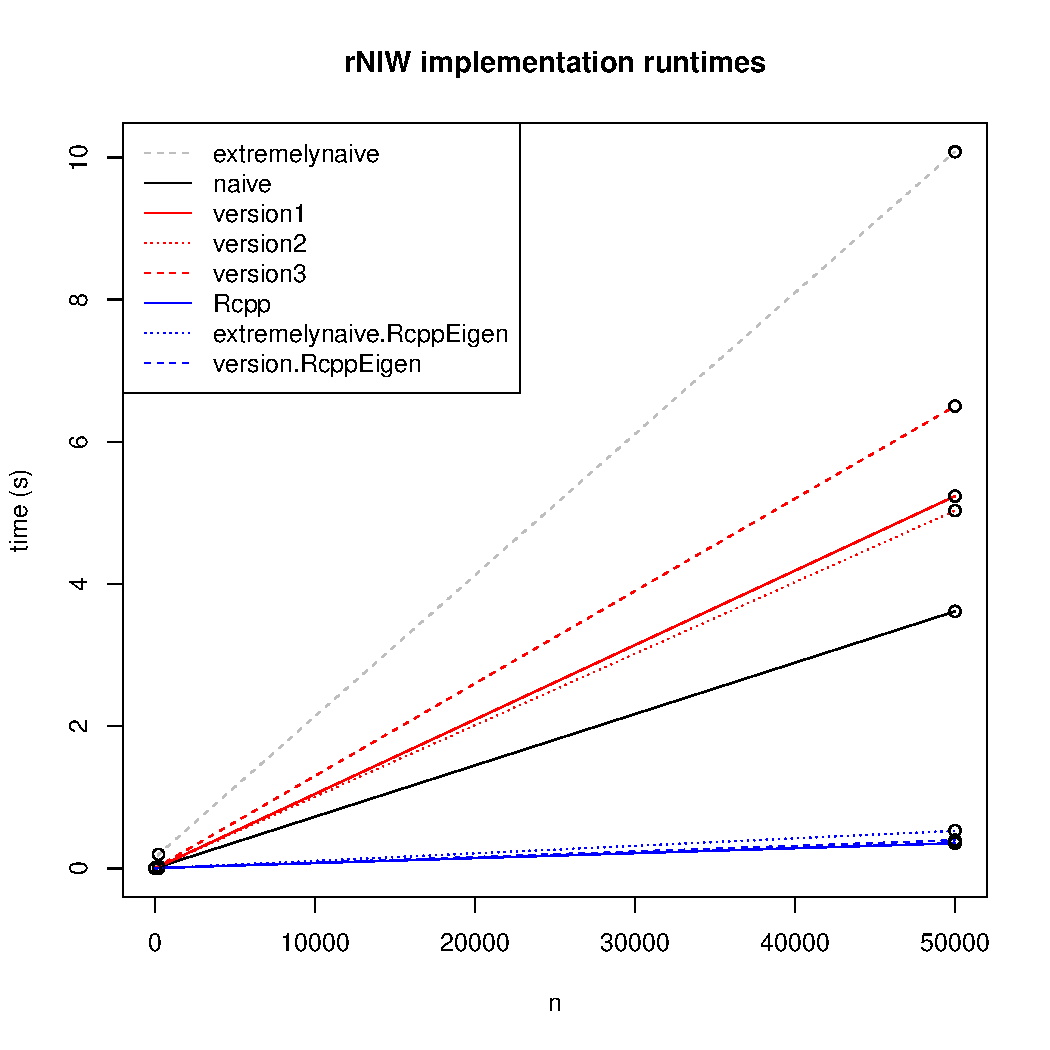
\includegraphics[scale=.7]{runtimes.pdf}\\*
\emph{Implementation runtimes. The naive algorithms are monochrome; the efficient algorithm prototyped in R is red; the C implementations (naive and efficient) are blue.}

As expected, the runtime is linear in $n$, since every sample of the $n$ is generated identically. We fit lines to each algorithm's runtime to estimate their scaling coefficient. We picked \emph{naive} as a baseline and put all algorithm frequencies on a relative scale.



\begin{center}
Runtime summary\\*
\begin{tabular}{rrrr}
    algorithm       & slope  &      ratio   &        sd\\
    \hline
              \emph{extremelynaive}   &4918.468  & 0.35 & 3.43e-05 \\
                \emph{version3}   &7648.601 & 0.55 & 1.82e-06 \\
               \emph{version1}   &9543.389 & 0.69 &2.57e-04 \\
                \emph{version2}   & 9980.602 & 0.72 & 1.54e-04 \\
                   \emph{naive}  &13890.529  & 1.00 & 7.27e-04 \\
  \emph{extremelynaive.RcppEigen} & 94128.482 & 6.78 & 3.96e-03 \\
        \emph{version.RcppEigen} & 125032.317  & 9.00 & 4.38e-03 \\
                     \emph{Rcpp} & 143356.322  & 10.32 & 3.97e-02 \\
    \hline
\end{tabular} \\*
 \emph{
    \emph{slope} is each algorithm's performance samples/second,
    \emph{ratio} is the ratio of each against "naive";
    \emph{sd} is the standard deviation of\emph{ratio}. Sorted in order of performance, worst to best.
    }
\end{center}

These results show that our algorithm gets about a 25 times times speed up over the extremely naive algorithm. But this is misleading: the naive algorithm that an R user would reach for would is not the deeply naive algorithm, but rather what we wrote as \emph{naive}, where we call out to R's built in \emph{rWishart} function. Compared to this version, our blazing fast best implementation is only 10 times better. The explanation is that almost all of the naive algorithm's output, the $n d^d$ entries of $V$, are constructed at the C level, because \emph{rWishart} is a native function. The sheer amount of time that this saves makes the naive algorithm faster than all of our R implementations of the efficient algorithm.

There is another unusual result: the algorithm written with more \emph{backsolve}s (\emph{version3}) is slower than the one without, even though \emph{backsolve} is a $O(d^2)$ algorithm and matrix multiply is $O(d^3)$ \cite{?????}. This might be an artifact of our only testing on small matrices, where a direct multiply is better, though.

% (4 pages?)
\Section{Application}

The NIW distribution is a extremely common conjugate prior. Here, we use our algorithm to rapidly do a simulation study.

% 1.25 pages
\Subsection{Multivariable Regression}

Linear regression $Y = X\beta + e$ with $e_i \sim N(0, \sigma^2)$ (i.i.d.) generalizes simple linear regression $y_i = b_1 x_i + b_0 + e_i$ so that $X$ becomes a matrix with one column per predictor variable. The goal of linear regression is to find the vector $\beta$ and the scalar $\sigma^2$.

The multivariable model is a further generalization which adds columns to $Y$ (and hence to $\beta$ as well). As before, each row of $Y$ is a single independent and identically distributed sample, but it is itself multivariate \textendash multivariate normal, in fact \textendash which means it has a whole covariance matrix $V$ associated with it. The goal of multivariable regression is to find the matrix $\beta$ which describes the linear relationships (if any) between the variates represented by the columns of $X$ and the variates represented by the columns of $Y$ which also getting an estimate of $V$.

Under Bayesian inference, the NIW distribution can be used to generate point estimates and credible intervals for $\beta$ and $V$. Here's how.\\

Let $X_{n\times p} = [x_{ij}]$ and $Y_{n\times q} = [y_{ij}]$ be matrices of $p$ predictors and $q$ responses for each of $n$ observations, and let $E_{n\times q}$ be the matrix of random errors. The full multivariable regression model is

\[Y = X\beta + E, E \sim MN_{q \times p}(0, I_d, V)\]

where $\beta_{p\times q} = [\beta_{ij}] $ and $V_{q\times q}$, and $MN$ is the \emph{Matrix Normal} distribution \cite{MatrixNormal}, which is a generalization of the gaussian distribution that produces whole matrices at once.

The conjugate prior for the model is:

\begin{align*}
	V &\sim  Inv-W_q(\Psi,\nu)\\
	\beta|V &\sim MN_{p \times q}(\Lambda, Omega^{-1}, V)
\end{align*}

The parameters of the prior are $\Psi_{q\times q}, \nu_{1\times 1}, \Lambda_{p\times q}, \Omega_{p\times p}$\\

The resulting posterior distribution is \cite{Lysy}

\begin{align*}
	V|Y,X &\sim  Inv\text{-}W_q(\Psi+S+C,\nu+n)\\
	\beta|V,Y,X &\sim MN_{p \times q}\{A\Lambda + (I-A)\hat{\beta}, V  \otimes (X'X +\Omega)^{-1}\}
\end{align*}
where 
\begin{align*}
\hat{\beta} &= (X'X)^{-1}X'Y\\
S &= (Y-X\hat{\beta})(Y-X\hat{\beta})\\ 
A &= (X'X + \Omega)^{-1}\Omega\\
C &= \hat{\beta}'(X'X)\hat{\beta} + \Lambda'\Omega\Lambda - (X'X\hat{\beta} + \Omega\Lambda)'(X'X+\Omega)^{-1}(X'X\hat{\beta} + \Omega\Lambda)
\end{align*}

The above means that given data $X$, $Y$, and the prior parameters, we have computable formulas for the parameters of the posterior--which is the estimated distribution of $\beta$ and $V$. We generalized our Normal Inverse Wishart sampler to a Matrix Normal Inverse Wishart sampler, and \emph{lm.multivariable} is a subroutine which uses it return samples of $B$ and $V$. Its code is in the appendix, and next section shows a usage example.

\Subsubsection{Boston housing data example}

Using the Boston housing data available in R's MASS library, we demonstrate \emph{lm.multivariable} by predicting 6 of the variates on the other 8\\

\begin{lstlisting}[frame=single, language=R]
require(MASS)
D <- Boston
Y <- D[c("crim", "zn", "indus", "tax", "black", "lstat")]
X <- D[c("chas", "nox", "rm", "age", "dis", "rad", "ptratio", "medv")]

# construct 100,000 samples from the posterior
# using flat priors for Psi and Kappa, and df=73
Result <- lm.multivariable(100000,as.matrix(X),as.matrix(Y))

# Now that we have that, we can generate 95% credible interval
#by generating lower and upper quantiles

apply(Result$B, c(1,2), quantile, probs = 0.025)
#        [,1]       [,2]        [,3]        [,4]       [,5]        [,6]
#[1,] -2.4726166 -5.8679744  0.09608906 -32.9824267 -11.281075 -1.55826198
#[2,] -6.9573162 -0.8674746 20.12296722 256.4240012  71.771290 12.86687197
#[3,]  0.6781378  1.6702512 -1.27047227  -2.1000956 -14.681060 -1.33368492
#[4,] -0.1553847 -0.4728362 -0.09345642  -1.6003269  -1.790386 -0.08581789
#[5,] -0.5264732  6.4092475 -0.97953076   0.1691556   8.454171  0.20377180
#[6,]  0.4767344  0.2930137  0.04739809  13.7503723  -5.358764 -0.03775675
#[7,] -0.1783143 -2.4605295  0.36683531   4.8444292  11.568813  0.34594612
#[8,] -0.2359186  0.1865307 -0.06683020  -1.3784741   3.828851 -0.31275303

apply(Result$B, c(1,2), quantile, probs = 0.975)
apply(Result$V, c(1,2), quantile, probs = 0.025)
apply(Result$V, c(1,2), quantile, probs = 0.975)

# Example with non-flat priors

q <- dim(Y)[2];
p <- dim(X)[2]

Psi <- diag(q);
df <- 100;
Lambda <- matrix(1, p,q);
Omega <- diag(p);

Result <- lm.multivariable(100000,as.matrix(X),as.matrix(Y), 
                    Psi = Psi, Lambda = Lambda, Omega = Omega, df  = df)
       
apply(Result$B, c(1,2), quantile, probs = 0.025)
apply(Result$B, c(1,2), quantile, probs = 0.975)
apply(Result$V, c(1,2), quantile, probs = 0.025)
apply(Result$V, c(1,2), quantile, probs = 0.975)


# Can also take a histogram to take a look a the distribution
# one example:

hist(Result$B[1,1,], breaks = 100, probability = TRUE)

\end{lstlisting}

\emph{lm.multivariable} is reusable. Any data table can be partitioned into $X$ and $Y$ columns and run through it to construct estimates of the relationship between the variates.

% .5 pages
\Section{Conclusion}

We implemented a Matrix-Normal-Inverse-Wishart sampler and proved its accuracy and speed. It is an improvement over what a lone R user would use before, but it is not as strikingly faster as we hoped. Still, it offers notable gains, and the multivariable regression algorithm is easy to use and totally general.\\

% Put stuff not yet done that we plan to do or wish we could do
We have ideas for improvement. There are other variants of the efficient algorithm we would like to try, especially ones invoking parallelization and GPUs.  Once the code is solid, wish to get this code to a production-ready state that could be uploaded to CRAN \cite{CRAN} \\

We offer this code \cite{MNIW} up in the hope it will make large linear models with an inverse-wishart prior tractable to the working statistician.



% 1 page
\newpage


\begin{thebibliography}{9}

\bibitem{R}R Core Team (2014). R: A language and environment for statistical computing. R Foundation for
  Statistical Computing, Vienna, Austria. URL http://www.R-project.org/.
  
\bibitem{Rcpp} Dirk Eddelbuettel and Romain Francois (2011). Rcpp: Seamless R and C++ Integration. Journal of
  Statistical Software, 40(8), 1-18. URL http://www.jstatsoft.org/v40/i08/.

\bibitem{RcppEigen}Douglas Bates, Dirk Eddelbuettel (2013). Fast and Elegant Numerical Linear Algebra Using the
  RcppEigen Package. Journal of Statistical Software, 52(5), 1-24. URL
  http://www.jstatsoft.org/v52/i05/.
\bibitem{MCMCpack}Andrew D. Martin, Kevin M. Quinn, Jong Hee Park (2011). MCMCpack: Markov Chain Monte Carlo in R.
  Journal of Statistical Software. 42(9): 1-21. URL http://www.jstatsoft.org/v42/i09/. 
 
\bibitem{LaplaceDemon}Statisticat, LLC. (2014). LaplacesDemon: Complete Environment for
  Bayesian Inference. Bayesian-Inference.com. R package version
  14.04.05. [http://www.bayesian-inference.com/software] 
 
\bibitem{MNIW}Daniel Galperin and Nick Guenther. (2014). MNIW. Version pre-alpha. [http://www.github.com/kousu/MNIW]
 
 \end{thebibliography}


\newpage
\newpage

\Section{Appendix}

\Subsection{rNIW Implementations}

For brevity, only the unique portions of each implementation are shown. See the full codebase \cite{MNIW} for the missing details.

%\Subsubsection{"Naive" implementations}

\begin{lstlisting}[frame=single, language=R]
  d = length(Mu)
  ans = rNIW.alloc(n,d)
  
  for(i in 1:n) {
     ans$V[,,i] = rInvWishart(1, df, Psi)[,,1];
     ans$X[,i] = rmvnorm(1, Mu, ans$V[,,i]/kappa);
  }
\end{lstlisting}
\emph{extremelynaive}


\begin{lstlisting}[frame=single, language=R]
  ans$X = matrix(NA, d, n)
  ans$V = rInvWishart(n, df, Psi);   
  
  # unfortunately, generating X must still be in a loop because each sample has a different distribution
  # and there's no way with rmvnorm to ask "give me n samples and here's the parameters for each"
  # ..is there?
  #
  for(i in 1:n) {
     ans$X[,i] = rmvnorm(1, Mu, ans$V[,,i]/kappa);
  }
\end{lstlisting}
\emph{naive}

\begin{lstlisting}[frame=single, language=C]
  unsigned int d = Mu.length();
  
  NumericVector V(Dimension(d,d,n));
  NumericVector X(Dimension(d,n));
  
  for(unsigned int i=0; i<n; i++) {
    NumericMatrix Vi = riwishart(Psi, df);

    for(int j=0; j<d; j++) {
    for(int k=0; k<d; k++) {
      V[d*d*i + j*d + k] = Vi(j, k);
    }
    }
    
    Vi = Rcpp::wrap(as<Map<MatrixXd> >(Vi) / kappa);
    NumericVector Xi = rmvnorm(1, Mu, Vi);
    for(int j=0; j<d; j++) {
      X[d*i + j] = Xi(j);
    }
    
  }
\end{lstlisting}
\emph{extremelynaive.RcppEigen}


\Subsubsection{"Efficient" implementations}

\begin{lstlisting}[frame=single, language=R]
BartlettFactor <- function(d, df) {
  A = matrix(nrow=d, ncol=d)
  A[,] = 0
  df = df-(1:d)+1
  diag(A) = sqrt(rchisq(d, df))
    
  # set the below-diagonals to N(0,1)s
  i_lower = col(A) > row(A)
  A[i_lower] = rnorm(sum(i_lower))
  
  A
}
\end{lstlisting}
\emph{BartlettFactor}, upon which the efficient algorithm is founded.


\begin{lstlisting}[frame=single, language=R]
  gamma.inv = solve(chol(solve(Psi)))
  for(i in 1:n) {    
    # construct the cholesky decomposition of a W(I, df) 
    A = BartlettFactor(d, df)
    
    A.inv = backsolve(A, I)
    U.inv = gamma.inv %*% A.inv
    
    ans$V[,,i] = tcrossprod(U.inv) #note well that this is not a LU decomposition -- it's UL
    
    # now we want X ~ N(Mu, V/kappa)
    z = rnorm(d); vector
    ans$X[,i] = Mu + U.inv %*% z/sqrt(kappa)
  }
\end{lstlisting}
\emph{version1}, the basic (should-be) efficient algorithm.


\begin{lstlisting}[frame=single, language=R]
  gamma.inv = solve(chol(solve(Psi)))
  for(i in 1:n) {
     
     A = BartlettFactor(d, df)
     A.inv = backsolve(A, I)
     
     z = rnorm(d);
     
     U.inv = gamma.inv %*% A.inv
     ans$V[,,i] = tcrossprod(U.inv)
     ans$X[,i] = U.inv %*% z
  }
  ans$X =  Mu + ans$X/sqrt(kappa) 
\end{lstlisting}
\emph{version2}, which uses R's vectorization syntax.


\begin{lstlisting}[frame=single, language=R]
  gamma = chol(solve(Psi))
  
  for(i in 1:n) {  #apply scaling after the fact
     
     A = BartlettFactor(d, df)
     
     U = A %*% gamma
     
     # sample V
     U.inv = backsolve(U, I) 
     ans$V[,,i] = tcrossprod(U.inv)
     
     # sample X
     z = rnorm(d);
     ans$X[,i] = backsolve(U, z)
  }
  ans$X =  Mu + ans$X/sqrt(kappa) 
\end{lstlisting}
\emph{version3}, which uses \emph{backsolve} instead of a normal matrix multiply.


\begin{lstlisting}[frame=single, language=R]
  # precompute some useful values
  d = length(Mu)
  gamma.inv = solve(chol(solve(Psi)))
    
  return(rNIW_Rcpp(n, d, Mu, kappa, gamma.inv, df))
\end{lstlisting}
\emph{Rcpp}, R side of the code.


\begin{lstlisting}[frame=single, language=C]
  NumericVector V_ans(Dimension(d,d,n));
  NumericVector X_ans(Dimension(d,n));
  
  
  NumericVector A(Dimension(d,d));
  for (int k = 0; k < n; k++){
  BartlettFactorCpp(d,df, A);
  NumericVector A_inv = backSolveInverse(A,d);
  
  NumericVector z = rnorm(d);
  
  
  NumericVector U_inv(Dimension(d,d));
  // compute upper triangular dot product
  for (int col = 0; col < d; col++){ // col of result 
    for(int row = 0; row < d; row++){ // row of result
      for(int i = 0; i < d; i++){
        U_inv[col*d+row] +=  gamma_inv[i*d + row] * A_inv[col*d + i];
      }
    }  
  }
  
  // compute crossprod(U_inv)
  for (int col = 0; col < d; col++){
    for (int row = 0; row < d; row++){
      for(int i = 0; i < d; i++){
        V_ans[k*d*d + col*d + row] += U_inv[i*d + row] * U_inv[i*d + col];  
      }
    }
  }
  
  for(int i = 0; i < d; i++){
    for(int j = 0; j < d; j++){
      X_ans[k*d+i] += U_inv[j*d + i]*z[j];
    }
      X_ans[k*d + i] = X_ans[k*d + i]/sqrt(kappa) + Mu[i];
  }
  
  }
\end{lstlisting}
\emph{Rcpp}, C side of the code


\begin{lstlisting}[frame=single, language=C]
  NumericVector V(Dimension(d,d,n));
  NumericVector X(Dimension(d,n));

  // invert Psi  
  MatrixXd Psi_inv = as<Map<MatrixXd> >(Psi).inverse();
  
  // factor Psi
  MatrixXd Gamma = Psi_inv.llt().matrixU();

  NumericVector A = NumericVector(Dimension(d,d));
  for(unsigned int i=0; i<n; i++) {
    // step 1: generate V
    BartlettFactorCpp(d, df, A);
    MatrixXd A_ = as<Map<MatrixXd> >(A);  //map into Eigen so we can use linear algebras
    MatrixXd U = A_*Gamma;
    MatrixXd U_inv = U.inverse();
    MatrixXd Vi = tcrossprod(U_inv);
    
    // memcpy the result out of Eigen and into Rcpp
    for(int j=0; j<d; j++) {
    for(int k=0; k<d; k++) {
      V[d*d*i + j*d + k] = Vi(j, k);
    }
    }
    
    // step 2: generate X
    VectorXd Xi = U.triangularView<Upper>().solve(as<Map<VectorXd> >(rnorm(d))); // backsolve(U, z)
    Xi /= sqrt(kappa);
    Xi += as<Map<VectorXd> >(Mu);
    for(int j=0; j<d; j++) {
      X[d*i + j] = Xi(j);
    }
    
  }
\end{lstlisting}
\emph{version.RcppEigen}




\Subsection{Multivariable Regression}

\begin{lstlisting}[frame=single, language=R]
lm.multivariable <- function(m, X, Y, Lambda=NULL, Omega=NULL, Psi=NULL, df=71) { # TODO: Not sure what to name this.
  # Multivariable Regression via Bayesian Reasoning
  # 
  # This fits the model Y = XB + E where (E_i)^T ~iid MultiNormal(0, V)
  #  but it doesn't fit it in the frequentist sense of constructing
  #  true values for B and V -- instead it produces samples from the
  #  Bayesian Posterior.
  # The posterior, like a good little bayesian, is conjugate in this case:
  #  both the prior and the posterior are Matrix-Normal|Inverse-Wisharts.
  #
  # args:
  #  m: the number of samples to take
  #  X, Y: the observed data; these should be (n,q) and (n,d)
  #  Psi, df, Lambda, Omega: your prior knowledge, encoded
  #    as parameters of the Normal|Inverse-Wishart distribution.
  #   You should provide a df (though this won't make a huge difference)
  #    but, for convenience, by default the other parameters are set
  #    to give "flat" (aka uninformative aka improper) priors. 
  #   The flat prior on Omega causes Lambda to be ignored
  #    (hence its default value: NULL), and, as a special exception,
  #    causes the degrees of freedom of the posterior to change
  #     from (df+n) to (df+n-d).
  #  The flat prior on Psi is orthogonal to the flat prior on Omega (XXX is this true? surely it has some effect, even if only numerical/speed/something)
  #  (the argument order is chosen to reflect the distribution,
  #  which is the result of sampling
  #      MatrixNormal(Lambda, Omega, InverseWishart(Psi, df)), 
  #   though it does makes calling this function awkward)
  # 
  # returns:
  #  a list containing the posterior samples:
  #   $B
  #   $V
  
  n <- dim(X)[1];
  stopifnot(n == dim(Y)[1])
  q <- dim(Y)[2];
  d <- dim(X)[2];
  
  # TODO: can add some checks here
  
  #X'X is used often, only time X is used by itself is in S
  X.sq <- crossprod(X)
  
  # this posterior is neat:
  # it actually involves taking the usual frequentist fit (as produced by lm())
  #  B = (X'X)^{-1}X'y
  # and trading off between that fit and the information from the prior.
  # So, compute the OLS fit beta.hat and its squared-error (SSE) S 
  beta.hat <- solve(X.sq, t(X) %*% Y);
  residuals <- (Y - X %*% beta.hat);
  S <- crossprod(residuals)
  
  # now incorporate the prior parameters
  # the flat priors are special-cased to avoid
  # numerical instability and R's thorny gorgon's type system
  
  if(is.null(Psi)) { Psi = 0 } #let scalar splaying sort it out
  
  if(is.null(Omega)) {
    mNIW.Mu <- beta.hat
    mNIW.Kappa <- X.sq;
    mNIW.Psi <- Psi + S;
    mNIW.df <- df + n - d;
  } else {
    
    if(is.null(Lambda)) {
      stop("You must specify Lambda if you use a non-flat prior on Omega");
    }
    
    # calculate kappa, also used in calculating C.
    # while C needs inverse, rMNIW already does the inverse, so not doing it here
    
    mNIW.Kappa <- X.sq + Omega;
    mNIW.df <- df + n - d;
    
    A <- solve(mNIW.Kappa, Omega);    
    I = diag(d) #identity matrix
    mNIW.Mu <- A %*% Lambda  +  (I-A) %*% beta.hat
    
    # could swap X'XB with XY, not sure if we should
    # this formula is long and grueling
    L = X.sq %*% beta.hat  + Omega %*% Lambda  #this term is used twice
    
    # in all lines below, mahalanobis gives this error 
    # Error in x %*% cov : non-conformable arguments
    C <- t(beta.hat) %*% X.sq %*% beta.hat
           # mahalanobis(beta.hat, 0, X.sq, inverted=TRUE)
             + t(Lambda) %*% Omega %*% Lambda
             #+ mahalanobis(Lambda, 0, Omega, inverted=TRUE) 
             - t(L) %*% solve(mNIW.Kappa) %*% (L);
             #- mahalanobis(L, 0, mNIW.Kappa);  #<-- more compact
             
    mNIW.Psi <- Psi + S + C;
  }
  
  # finally, do the heavy lifting given these posterior parameters
  result = rMNIW.Rcpp(m, mNIW.Mu, mNIW.Kappa, mNIW.Psi, mNIW.df)
  
  # rename the posterior samples to match the API
  names(result)[names(result) == "X"] = "B" 
  
  return(result)
}

\end{lstlisting}

\end{document}
